\documentclass[titlepage]{article}
\usepackage[tc]{titlepic}
\usepackage{graphicx}
\usepackage{amsmath}
\usepackage[top=25mm, bottom=25mm, left=27mm, right=27mm]{geometry}
\usepackage{caption}
\usepackage{listings}
\usepackage{lstlangarm}
\usepackage{tabu}
\usepackage[outdir=./]{epstopdf}


\date{}
\author{Erdal Sidal Dogan\\ \#041702023  \and Alp
	Gokcek \\ \#041701014}
\title{\includegraphics[width=0.6\textwidth]{../images/logo_en_color.png}\\ 
\vspace{5em}
EE306 - Microprocessors\\
\vspace{2em}
\textbf{Laboratory Exercise 3 \linebreak Subroutines
}\\
\vspace{1.5em}
March 17, 2020}

\begin{document}
	\maketitle
	\section{Sigma Sum}
	In this experiment we wrote an assembly program that finds the mean of given set of numbers, length of the number sequence is defined as $N$. Listing \ref{part3code} below calculates the result of the following expression $\sum_{i=0}^{N}i$\\
	
	First step is to store the value that we are going to sum up to $(N)$ in the R0 register. Then, we load $0$ to the R1. It will be used as temporary register during the summation process, later on we will move the value of the R1 to the R0 since it has been specifically requested to store the result in R0. \\
	
	Subroutine \texttt{FINDSUM} adds current value of R1 to R0, then decreases the value of the R0 by 1. Finally, checks if the R0 is equal to 0. If no; repeats the same sequence. If yes; it's job is done. After \texttt{FINDSUM} finishes its operation, we move the result from R1 to R0 and end the program.
	
	\lstinputlisting[language={[ARM]Assembler}, frame=single, basicstyle=\ttfamily, caption=Assembly Code for Sigma sum \& calculating average]{../source_codes/task-iii.s} \label{part3code}
	
	\begin{figure}[h]
		\centering
		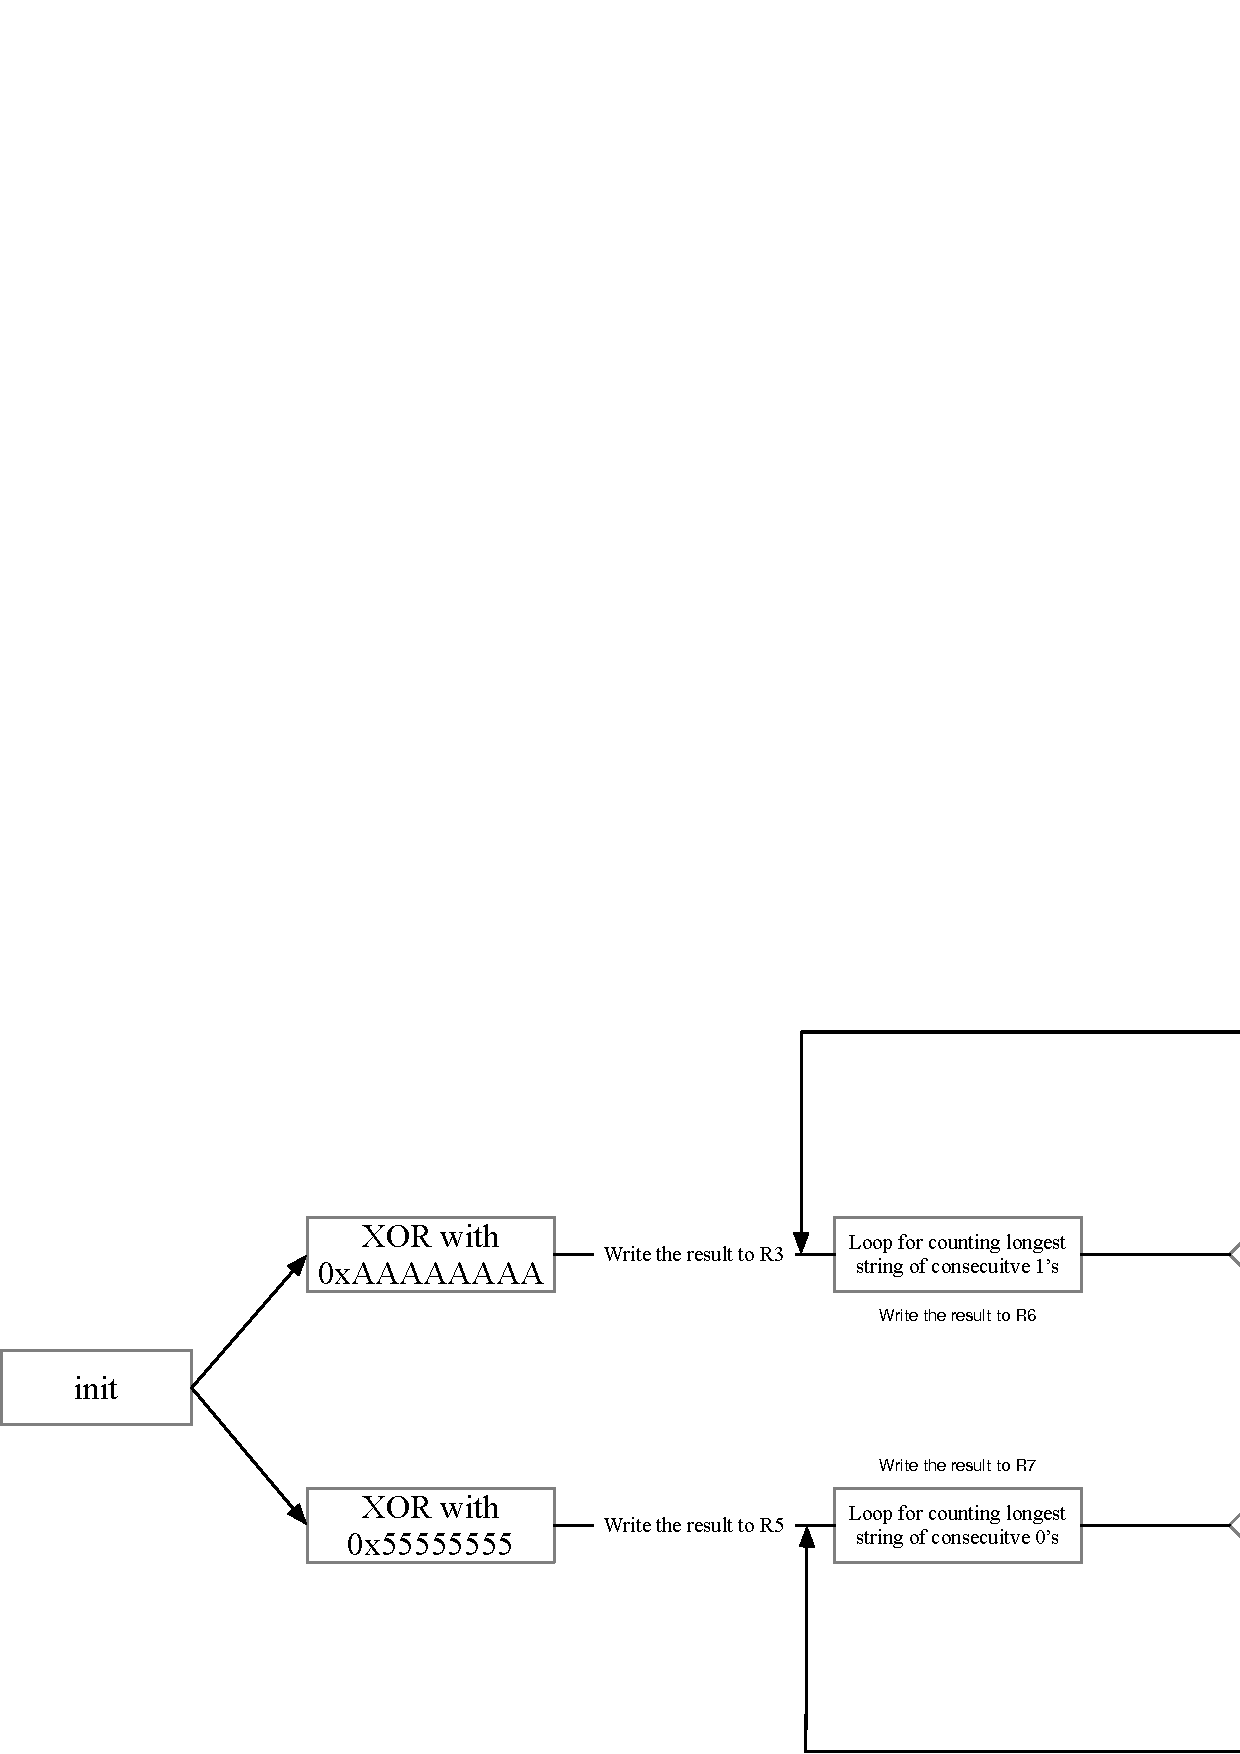
\includegraphics[scale=.45]{../images/task-iii.pdf}
		\caption{Flowchart of the Listing \ref{part3code}}
	\end{figure}
	
	\newpage
	\section{Part IV - Bubble Sort}
	In this experiment we wrote an assembly program that sorts the given numbers using bubble sort algorithm. First step is to create a pointer to the memory location that will be sorted and after that load the number of values that will be sorted which placed as the first element of that memory location. Then, we create a pointer to the first element of the list that will be sorted and then we started the sorting subroutine.\\
	In the sorting subroutine's initialization part, we save the link register's value for one time then save the content of R0 and R1 and update the value of flag register as 0. Flag register is used for checking whether any item is sorted on that traverse. After initialization, algorithm checks whether we traversed the whole list or not. If we traversed the whole list, then we branch to checking part. If not, algorithm loads 2 items to be compared from memory and check whether first element is greater or equal to second element. If yes, continue to traverse, else, start swapping subroutine. If no, continue to traverse.\\
	In swapping subroutine, we store the first element in second elements memory location and store second element in first elements memory location. Then, we update the status flag and return to sorting subroutine.\\
	On checking part, we restore the content of R0 and R1 and decrement R1 which holds the number of elements. After that, we check whether we swapped anything on that traverse. If yes, branch to sorting subroutine, else, restore link register and update R0 to hold the first elements position on memory.
	\lstinputlisting[language={[ARM]Assembler}, frame=single, basicstyle=\ttfamily, caption= Assembly code for bubble sort algorithm]{../source_codes/task-iv.s} \label{part4code}
		
	\begin{figure}[h]
		\centering
		\includegraphics[scale=.45]{../images/task-iv.pdf}
		\caption{Flowchart of the Listing \ref{part4code}}
	\end{figure}

\end{document}